\chapter{Entscheidungsbaum basierte Handgestenerkennung}
Entscheidungsbäume sind sehr schnell im Vergleich zu neuronalen Netzen. Allerdings eignen sich neuronale Netze oft besser für komplexe ML Probleme, da sie leicht zu konstruieren sind
und bereits auf Rohdaten gut generalisieren. Das untersuchte Problem weißt aber nur eine geringe Komplexität. Aus diesem Grund wird untersucht, ob Entscheidungsbaum basierte Klassifizierer
eine ausreichende Erkennungsgenauigkeit erzielen.

\section{Modell}
Insgesamt werden 22528 verschiedene Konfigurationen getestet. Sie unterscheiden sich in der Baumgröße, Waldgröße, Featureauswahl, Ensemble-Methode und Blattgröße.
\newline
\begin{figure}
    \centering
    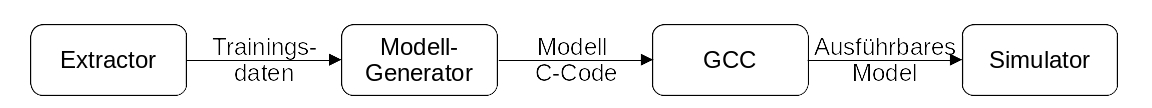
\includegraphics[width=\linewidth]{images/model_workflow.jpg}
    \caption{Arbeitsablauf um ein Model zu trainieren und zu validieren.}
    \label{fig:model_workflow}
\end{figure}
\newline
Jeder Entscheidungswald wird mit dem Python-Modul \texttt{Scikit-Learn} trainiert. Scikit-Learn implementiert den Konstruktionsalgorithmus CART (siehe Sektion \ref{sec:construction}) für den Entscheidungsbaum und bietet
zusätzlich zahlreiche Ensemble-Methoden an. Jede Konfiguration folgt dem in Abbildung \ref{fig:model_workflow} illustrierten Arbeitsablauf.
\newline
\newline
Zunächst wird die Trainingsmenge vorverarbeitet. Dabei werden die verschiedenen
Features extrahiert, die während der Konstruktion eines Entscheidungsbaumes benötigt werden. Dann wird das Model mit Scikit-Learn und den gegebenen Konfigurationsparametern generiert. Anschließend wird aus dem Model
ausführbarer C-Code generiert und kompeliert. Zuletzt wird die Erkennungsgenauigkeit des ausführbaren Models auf der Testmenge von Klisch, der Gestentestmenge und Nullgestentestmenge ermittelt.

\subsection{Training}
\label{sec:Training}
Mit Scikit-Learn werden Wahl basierte Entscheidungswaldklassifizierer mit den in Sektion \ref{sec:Ensemble} genannten Ensemble-Methoden trainiert. Insgesamt werden Waldgrößen zwischen 1 und 16 betrachtet und
Maximalhöhen von den einzelnen Entscheidungsbäumen zwischen 1 und 22. Außerdem werden die Blattgrößen, d. h. die minimale Anzahl von Trainingsdateneinträgen pro Blatt, \textit{1, 2, 4 und 8} untersucht.
\newline
\newline
Der letzte Parameter verringert potentiell die Erkenneungsgenauigkeit von den einzelnen Entscheidungsbäumen, verringert aber auch die Größe des Baumes signifikant.
Dadurch können Entscheidungswälder gefunden werden, die zuvor nicht in den Programmspeicher eines Arduino Boards gepasst haben (siehe Sektion \ref{sec:eval_size}).
\newline
\newline
Die Konstruktion der Entscheidungswälder ist nicht deterministisch. Zuallererst muss die Konstruktion eines einzelnen Entscheidungsbaumes nicht deterministisch sein, da selbst wenn immer die beste Teilung
ausgewählt wird, können mehrere Teilungen auch gleich gut sein. Aus den gleich guten Teilungen müsste zufällig eine ausgewählt werden. Folglich ist jede Ensemble-Methode zufällig. Außerdem wählt die RandomForest-Methode
zufällig eine Featureauswahl, und die Bagging-Methode partitioniert die Trainingmenge zufällig. Aus diesem Grund kann in Scikit-Learn ein \texttt{random\_state} zugewiesen werden, der den \textit{Seed} des
unterliegenen Zufallszahlengenerators setzt.
\newline
\newline
Dementsprechend kann man die Konstruktion als Monte Carlo Methode betrachten, d. h. wiederholte Ausführungen erhöhen die Wahrscheinlichkeit, dass das beste Ergebnis dieser Konfiguration gefunden wurde.
Jede Konfiguration wird aus diesem Grund mit 140 verschiedenen \texttt{random\_state} ausgeführt.

\subsection{C-Code Generierung eines Entscheidungsbaumes}
\label{sec:cCodeTree}
Das Model soll auf kleinen eingebetteten Systemen ausgeführt werden. Diese haben eine Toolchain um die Firmware zu generieren, die meistens auf der Programmiersprache \texttt{C} basiert. Dies trifft auch auf das in
dieser Arbeit benutzten Arduino Board zu.
\begin{lstlisting}[label=lst:sklearnTreeStructure,caption={Skizze der rekursiven Datenstruktur für Entscheidungsbäume die von Scikit-Learn genutzt wird.}]
enum Knoten<T> {
    Blatt(Vec<usize>),
    Elternknoten {
        test: (features: Vec<T>) -> bool,
        knoten_links: Knoten<T>,
        knoten_rechts: Knoten<T>
    }
}
\end{lstlisting}
Das Model wird mit dem Python-Modul Scikit-Learn generiert. Dementsprechend muss aus der internen Repräsentierung von Scikit-Learn das Model extrahiert werden. Scikit-Learn definiert eine rekursive Datenstruktur in
der jedes Blatt für jede Klassifizierungsklasse die Anzahl der Trainingsdateneinträge enthält, die nach dem traversieren aller Test in diesem Blatt eingeordnet werden. Jeder Elternknoten besteht aus einem Test der
ein Feature mit einem Schwellenwert vergleicht und einen Knoten für jedes Ergebnis dieses Tests (siehe Listing \ref{lst:sklearnTreeStructure}). Im Falle von Scikit-Learn ist der der Test immer
ein $\leq$ Vergleich, weswegen es genau zwei Kindknoten gibt.
\begin{lstlisting}[label=lst:sklearnCCodeParent,caption={C-Code eines Elternknotens.}]
if (features[k] <= X) {
    Traversiere linkes Kind...
} else {
    Traversiere rechtes Kind...
}
\end{lstlisting}
Ein Elternknoten wird dementsprechend als ein \texttt{if (test) \{ \ldots\ \} else \{ \ldots\ \}} Ausdruck modeliert (siehe Listing \ref{lst:sklearnCCodeParent}). Dabei ist der \texttt{test} ein $\leq$ Vergleich eines
Features mit einem Schwellenwert und der Inhalt der einzelnen Blöcke ist abhängig von den Kindesknoten.
\begin{lstlisting}[label=lst:sklearnCCodeLeaf,caption={C-Code eines Blattes.}]
result[0] = (Anzahl Klasse 1) / (Gesamtanzahl im Blatt);
...
result[N] = (Anzahl Klasse N) / (Gesamtanzahl im Blatt);
return;
\end{lstlisting}
Der C-Code im Blatt ist abhängig von dem Wahlklassifizierer. Es können entweder die Klasse ausgewählt werden, die von den meisten Bäumen klassifiziert wurde, oder die
Erkennungswahrscheinlichkeiten jedes Baumes im Ensamble wird summiert und davon wird die Klasse mit der größten Summe ausgewählt (siehe Sektion \ref{sec:wahlklassifizierer}).
In dieser Arbeit wurde sich für letzteres entschieden. Im C-Code wird das modeliert durch die Zuweisung der Wahrscheinlichkeiten der einzelnen Klassen im Blatt zu dem Ergebnisparameter
\texttt{result} (siehe Listing \ref{lst:sklearnCCodeLeaf}).

\subsection{C-Code Generierung eines Entscheidungswaldes}
Ein Entscheidungswald besteht aus einem Ensemble von Entscheidungsbäumen. Bei der Evaluierung eines Entscheidungswaldes wird jeder Entscheidungsbaum evaluiert und die Ergebnisse zusammengefasst, z. B.
durch einen Wahlklassifizierer.
\begin{lstlisting}[label=lst:sklearnCCodeTreeFunction,caption={C-Code Funktionskopf eines Baumes $i$.}]
function tree_i(float* features, float* result);
\end{lstlisting}
Zunächst wird jeder Entscheidungsbaum als Funktion isoliert (siehe Listing \ref{lst:sklearnCCodeTreeFunction}). Als Eingabeparameter dienen die extrahierten Features und ein \texttt{float}-Array \texttt{result}, dass das
Ergebnis speichert.
\begin{lstlisting}[label=lst:sklearnCCodeTreeVoting,caption={C-Code des Wahlklassifizierers mit $N$ Klassen und $K$ Bäumen.}]
float tree_res[N] = { 0.0, ..., 0.0 };
float total_res[N] = { 0.0, ..., 0.0 };
unsigned char result_map[N] = { ... };

// Wiederhole dies für K Bäume
tree_i(features, tree_res);
total_res[0] += tree_res[0];
...
total_res[N-1] += tree_res[N-1];

unsigned char max_index = 0;
float max_value = 0;
for (unsigned char i = 0; i < N; ++i) {
    if (max_value < total_res[i]) {
        max_value = total_res[i];
        max_index = i;
    }
}
return result_map[max_index];
\end{lstlisting}
Listing \ref{lst:sklearnCCodeTreeVoting} zeigt wie ein Ensemble bestehend aus $K$ Entscheidungsbäumen, die jeweils $N$ mögliche Klassifizierungsergebnisse zurückgeben. Diese werden mit einem Wahlklassifizierer
zusammengefasst. Zunächst wird jeder Baum evaluiert und die Ergebnisse summiert. Anschließend wird die Klasse mit dem maximalen Wert zurückgegeben.
\section{Features}
Features bilden die Eingabe für einen Entscheidungsbaum. Gute Features sind integral, damit der Entscheidungsbaum gut generalisiert. Wenn die Featuremenge keine eindeutige Trennung der Klassen in der
Trainingsmenge zulässt, so ist auch keine gute Generalisierung zu erwarten.
\newline
\newline
In dieser Arbeit muss die Richtung der Handgeste klassifiziert werden. Die Handgeste kann mit verschiedenen Geschwindigkeiten und unterschiedlichen Distanzen zur Kamera durchgeführt werden. Mit
zunehmender Entfernung nimmt der Kontrast ab, da Streulicht einen größeren Einfluss hat. Für eine gute Generalisierung sollten die Features Invarianten zur Geschwindigkeit und den
Lichtverhältnissen haben. Erschwerend ist, dass die Handgeste nie exakt gleich ausgeführt wird. Sie kann leichte Kreisbewegungen aufweisen oder schräg durchgeführt werden, sodass einige
Fotowiderstände nicht verdeckt werden.
\subsection{Feature Verbesserungen}
Einige Anforderungen, können durch spezielle Änderungen an einem Feature ergänzt werden. Dazu gehören relative Helligkeitsunterschiede, Positionsinformationen und Entwicklung über die Zeit.
\newline
\newline
Relative Helligkeitsunterschiede können durch Normalisierung über die lokale Gesamthelligkeit eliminiert werden. Dadurch ändert sich aber die Art der Aussage über die absolute Helligkeit
zu einer Aussage über die relative Helligkeit. Das heißt, jeder Pixel in einem Bild wird durch die Summe der Pixel im Bild geteilt. Dies erzeugt eine Invarianz gegenüber der skalierten Helligkeiten,
jedoch nicht gegenüber Helligkeiten auf denen ein Offset addiert wurde.
\newline
\newline
Informationen über die Position können einerseits aus dem Argument des Features und andererseits durch partielle Anwendung inferiert werden. Beim Argument eines Features wird das Argument als Feature
bereitgestellt, indem das Feature bestimmte Bedingungen erfüllt. Bei $\arg(\max X)$ zum Beispiel, wird der Index bereitgestellt, an dem die Menge $X$ maximal ist. Bei der partiellen Anwendung wird das Feature auf
Teilmengen der Definitionsmenge angewendet und damit mehrfach zur Feature-Menge hinzugefügt, z. B. bei der Fotowiderstandmatrix könnten Zeilen und Spalten Teilmengen sein.
\newline
\newline
Die Entwicklung über Zeit kann ebenfalls über die Duplizierung des Features dargestellt werden. Anstatt einen einzelnen Bild zu unterteilen, wird die Handgeste in Zeitfenster aufgeteilt. Jedes Zeitfenster
fasst die einzelnen Bilder zu einem Bild zusammen. Für jedes Zeitfenster wird das Feature berechnet.
\subsection{Featureauswahl}
Insgesamt wurden 28 Varianten von Feature untersucht und davon 3 Feature verstärkt aus denen 20 Varianten entstanden sind. Die Features, die von Song et al. genutzt wurden
(siehe Tabelle \ref{tab:songFeatures}) eignen sich ohne Änderungen nicht, da sie mindestens eine Anforderung nicht erfüllen.
\newline
\newline
Mit dem \textit{Mean absolute value} ermöglicht es die einzelnen Handgesten zu unterscheiden, wenn das Feature in verschiedene Zeitfenster aufgeteil wird. Zusätzlich kann die Helligkeit normalisiert werden.
Um die Featuremenge zu verringern, können Spalten und Zeilen zusammengefasst werden. Allerdings generalisierte der Ansatz nicht gut, da die Varianz sehr groß ist durch die fehlende Invarianz zur Geschwindigkeit.
\newline
\newline
\textit{Average amplitude change} eignet sich gut um horizontale und vertikale Bewegungen zu unterscheiden. Allerdings ist es nicht möglich symethrische Bewegungen zu unterscheiden. Nicht untersucht wurden
Änderungen, die beim \textit{Mean absolute value} durchgeführt wurden.
\newline
\newline
Feature 2, 5, 7 bis 9 wurden nicht weiter untersucht weil sie zu komplexe Berechnungen bedürfen für das Arduino Board.

\subsubsection{Motion History}
Die Motion History zeigt eine Bewegunghistorie, indem kürzlich stattgefundene Bewegung heller ist als länger zurückliegende. Es ist invariant gegenüber Lichtverhältnisse, hat jedoch 2 große Schwachpunkte.
Einerseits kann es überlappende Bewegungen nicht richtig anzeigen, da eine kürzlich detektierte Bewegungung den Wert auf den Maximalwert $\tau$ setzt. Dies stellt in diesem Anwendungsfall kein
Problem dar, da die definierten Handgesten keine Überlappung erzeugen.
\newline
\newline
Andereseits ist das Feature bei konstantem $\tau$ und $\delta$ nicht Invariant gegenüber Geschwindigkeit. Als Lösung wurde $\delta$ abhängig von der Gestenlänge gemacht,
d. h. $\delta = \frac{\tau}{\#Bilder}$. Mit dieser Konfiguration ist die Bewegung nicht unvollständig, wenn sie langsam ausgeführt wird. Allerdings geht dieser Ansatz von einer konstanten
Ausführungsgeschwindigkeit der Handgeste aus.
\newline
\newline
Eine Bewegung in einem Pixel $q$ wird duch die Funktion \ref{formular:motion_history_phi} signalisiert, d. h. die Bewegung in $q$ findet statt, wenn eine Veränderung oberhalb des Durchschnitts detektiert wird.
\begin{align}
    \phi(q,t) = \begin{cases}
                    1 & if \Delta_{q,t} \geq \frac{1}{N} \sum_{n=1}^N \Delta_{q,n} \\
                    0 & otherwise
    \end{cases}
    \hspace{0.5cm}where\ \Delta_{q,t} = |q_t - q_{t-1}|
    \label{formular:motion_history_phi}
\end{align}

\subsubsection{Helligkeitsverteilung}
Ein Pixel $q$ ist am hellsten unter allen Pixeln in einem Bild $Q$, wenn $q$ den höchsten Wert hat. Analog ist der dunkelste Pixel, der mit dem geringsten Wert. Folglich kann der hellste Pixel als
$q' = \arg(\max Q)$, bzw. der dunkelste Pixel als $q' = \arg(\min Q)$ definiert werden.
\newline
\newline
Weiterhin wird die Bildsequenz in eine bestimmte Anzahl von gleich großen Zeitfenstern aufgeteilt. In jedem Zeitfenster wird der hellste bzw. dunkelste Pixel ermittelt. Aus der daraus resultierenden
Featuremenge kann jede definierte Handgeste inferiert werden. Sie ist invariant zu Lichtverhältnissen und Geschwindigkeiten. Per Definition gibt sie Auskunft über die Entwicklung über Zeit und die Position.
\newline
\newline
Es gibt mehrere Möglichkeiten die einzelnen Pixel in einem Zeitfenster zusammenzufassen.
\begin{itemize}
    \item Wähle das Minimum bzw. Maximum.
    \item Projeziere die Pixel auf ein kartesisches Koordinatensystem und fasse die Punkte über eine Abstandsmetrik zusammen, z. B. über den euklidischen Abstand.
    \item Unterteile die Pixel in Quadranten und wähle den Quadranten, der die meisten Einträge hat.
\end{itemize}
Außerdem können die Anzahl der Zeitfenster variiert werden und Pixel zu Gruppen zusammengefasst werden, d. h. Spalten und Zeilen.

\subsubsection{Schwerpunktverteilung}
\begin{figure}
    \centering
    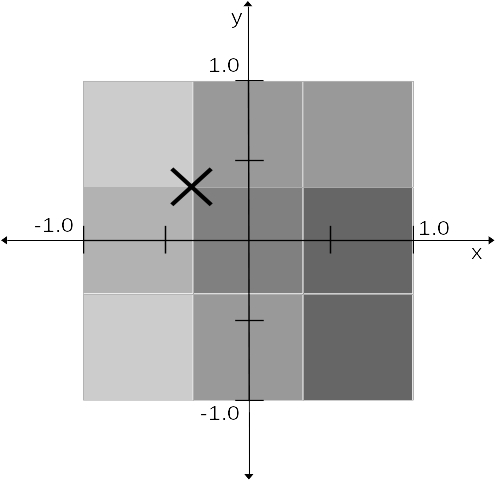
\includegraphics[width=0.5\linewidth]{images/schwerpunkt_ansatz.jpg}
    \caption{Illustration des Schwerpunktes im 3x3 Fotowiderstand-Array.}
    \label{fig:schwerpunkt}
\end{figure}
\begin{align}
    Q = \begin{pmatrix}
            q_{00} & q_{01} & q_{02} \\
            q_{10} & q_{11} & q_{12} \\
            q_{20} & q_{21} & q_{22}
    \end{pmatrix}
    \label{formular:pictureAsFormular}
\end{align}
Der Schwerpunkt $(X_Q, Y_Q)$ in einem Bild $Q$ (\ref{formular:pictureAsFormular}) ist über die Helligkeit in den einzelnen Pixel definiert. Der Pixel $q_{11}$ bildet den Nullpunkt des Koordinatensystems.
Dann ist relativ zur Gesamthelligkeit $P = \sum_{i,j} q_{i,j}$, $X_Q=\frac{\sum_{i=0}^{2} q_{i,2} - \sum_{i=0}^{2} q_{i,0}}{P}$ die horizontale Komponente
und $Y_Q = \frac{\sum_{i=0}^{2} q_{0,i} - \sum_{i=0}^{2} q_{2,i}}{P}$ die vertikale Komponente des Schwerpunktes \cite{schwerpunktAnsatz}.
\newline
\newline
Ähnlich zur Helligkeitsverteilung wird das Feature mit einer Zeithistorie erweitert durch die multiple Anwendung auf verschiedene Zeitfenster, wobei die Anzahl der Zeitfenster variiert werden kann. Die
einzelnen Schwerpunkte innerhalb eines Zeitfensters werden über den Durchschnitt zusammengefasst.
\newline
\newline
Sollte die Anzahl der Bilder einer Handgeste ein Vielfaches von der Anzahl der Zeitfenster sein, wird die gleiche Anzahl an Bilder auf jedes Zeitfenster verteilt. Ansonsten werden Überschüsse einem Muster
nach bestimmten Zeitfenstern zugeordnet. Bei 5 Zeitfenstern wird der erste Überschuss dem letzten Zeitfenster zugeordnet, der zweite dem ersten, der dritte dem dritten, der vierte dem zweiten.
\newline
\newline
Die Schwerpunktverteilung ist durch die Dividierung mit $P$ invariant gegenüber Skalierung der Helligkeit, jedoch nicht gegenüber einen Offset.

\section{Erstellte Werkzeuge und Bibliotheken}
\label{sec:recorder}
\begin{figure}
    \centering
    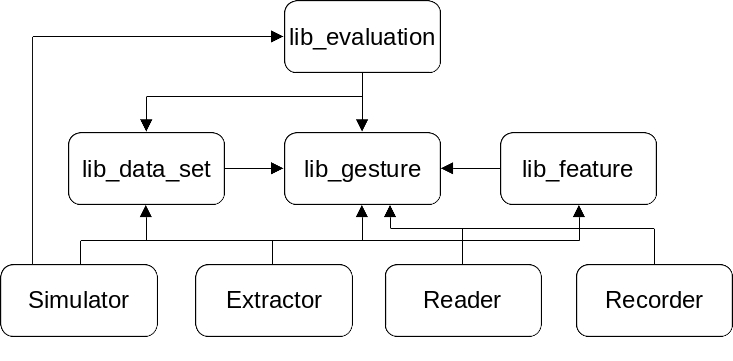
\includegraphics[width=0.75\linewidth]{images/architecture_overview.jpg}
    \caption{Abhängigkeitein der einzelnen Module.}
    \label{fig:architecture_overview}
\end{figure}
In dieser Arbeit mussten viele Features und Konfigurationen der Entscheidungsbäume untersucht und zu getestet werden. Aus diesem Grund wurde eine umfangreiche Infrastruktur geschaffen, die die
Auswertung von ML Modellen mit den Handgestendaten vereinfacht. Die Infrastruktur umfasst ein Datenmodel für Handgesten und kann die Datenmengen mit verschiedenen Parsingmethoden einlesen.
\newline
\newline
Außerdem können synthetischen Daten auf verschiedene Arten generiert werden. Die Architektur der Infrakstruktur erlaubt es weitere Features hinzuzufügen, ohne Kompatibilitätsprobleme zu verursachen.
Alle Funktionalitäten sind in Code-Bibliotheken isoliert, um die Integration in Hilfprogramme zu vereinfachen (siehe Abbildung \ref{fig:architecture_overview}).
\newline
\newline
Im folgenden wird die Funktionalität der einzelnen Module vorgestellt und die daraus erstellten Hilfsprogramme.
\newline
\newline
\texttt{lib\_gesture} definiert die Handgeste und die vorhandenen Gestentypen. Außerdem implementiert sie zwei Parsing-Methoden. Die erste Methode parsed Handgesten nach Annotation und die
zweite nach Kubiks Algorithmus (siehe Sektion \ref{sec:gesture_extraction}). Die Handgeste selber implementiert Methoden um synthetische Daten zu generieren.
\begin{itemize}
    \item Rotation um 90°, 180° und 270°.
    \item Nullgesten durch das Kombinieren der ersten Hälfte der Ausgangsgeste und der zweiten Hälfte von dessen Rotationen.
    \item Verschiebung der Pixel nach Oben und Unten für eine Links nach Rechts bzw. Rechts nach Links Geste und analog dazu eine Verschiebung nach Links und Rechts für die restlichen Handgesten.
    \item Rotation der äußeren Pixel um Diagonale Handgesten zu generieren.
\end{itemize}
\begin{lstlisting}[label=lst:FeatureInterface,caption={Interface, um ein Feature zu implementieren.}]
pub trait Feature {
    fn calculate(gesture: &Gesture) -> Self where Self: Sized;
    fn marshal(&self) -> String;
}
\end{lstlisting}
\texttt{lib\_feature} bietet ein einfaches Interface an um Feature mit einer Handgeste (siehe Listing \ref{lst:FeatureInterface}) zu implementieren. Zurzeit sind 28 verschiedene Feature implementiert.
\newline
\newline
\texttt{lib\_data\_set} stellt alle verfügbaren Datenmengen als statische Importe bereit. Einträge sind bereits nach Distanz zur Kamera, Helligkeit, Verdeckungsobjekt und Ausführungsgeschwindigkeit klassifiziert. Ein
Eintrag kann in der Helligkeit verändert werden entweder durch einen Offset oder indem er skaliert wird.
\newline
\newline
\texttt{lib\_evaluation} bietet ein Hilfsobjekt an, dass Datenmengen nach Erkennungsgenauigkeit auswertet und Berichte daraus generiert.
\newline
\newline
Der \texttt{Simulator} ist zweigeteilt. Der aktive Teil nutzt die die Gestenkandidatenerkennungsmethode nach Kubik, die in \texttt{lib\_gesture} implementiert ist, um den seriellen Datenstrom des Arduino zu parsen. Der
Gestenkandidat wird anschließend durch das hinterlegte Model klassifiziert und das Ergebnis ausgegeben. Der passive Teil evaluiert die Erkennungsgenauigkeit aller definierten Datenmengen.
\newline
\newline
Der \texttt{Extractor} extrahiert aus spezifizierten Datenmengen die definierten Features und exportiert diese in Dateien, sodass sie von dem Model zum Trainieren genutzt werden können. Optional kann die Datenmenge durch
sythetische Daten erweitert werden.
\newline
\newline
Der \texttt{Reader} gibt den seriellen Datenstrom des Arduino aus.
\newline
\newline
Der \texttt{Recorder} nutzt ähnlich wie der \texttt{Simulator} den seriellen Datenstrom des Arduino und die Parsingmethode von Kubik um Gestenkandidaten zu erkennen.
Diese Information wird genutzt, um in eine vordefinierte Datei die Handgesten reinzuschreiben. Um effizient Gesten aufzunehmen wurde der Ansatz von Kubik aufgegriffen mit
einem Gestentyp zu starten und folgend immer zwischen dem Inverstyp hin und her zu wechseln \cite{venzkeArticle}.
\newline
\newline
Das Programm wurde um zwei weitere Optionen erweitert. Mit der ersten Option wird immer nur eine bestimmte Handgeste hintereinander aufgenommen. Mit der zweiten Option wird jedes mal wenn eine Handgeste erkannt wurde,
der Gestentyp zur manuellen Eingabe erfragt. Mit disem Programm wurde die Datenmenge \texttt{DymelData} in wenigen Stunden erstellt (siehe Sektion \ref{sec:DymelData}).
\section{Aufgenommene Datenmenge}
\label{sec:DymelData}
\texttt{DymelData} ist eine Datenmenge, die mit dem \texttt{Recorder} (siehe Sektion \ref{sec:recorder}) erstellt wurde. Sie umfasst insgesamt 14410 Gesten in unterschiedlichen Konfigurationen. Sie wurde
einerseits aufgenommen, um unter den vorort bestehenden Lichtverhältnissen die Modelle miteinander vergleichen zu können und andererseits, um Test- und Trainingsdaten für Nullgesten bereitzustellen. In den
bisherigen Datenmengen enthält nur ein geringer Anteil Nullgesten.
\newline
\newline
\subfigbox{
\subfigure[Geringe Helligkeit]{\label{subfig:light_low}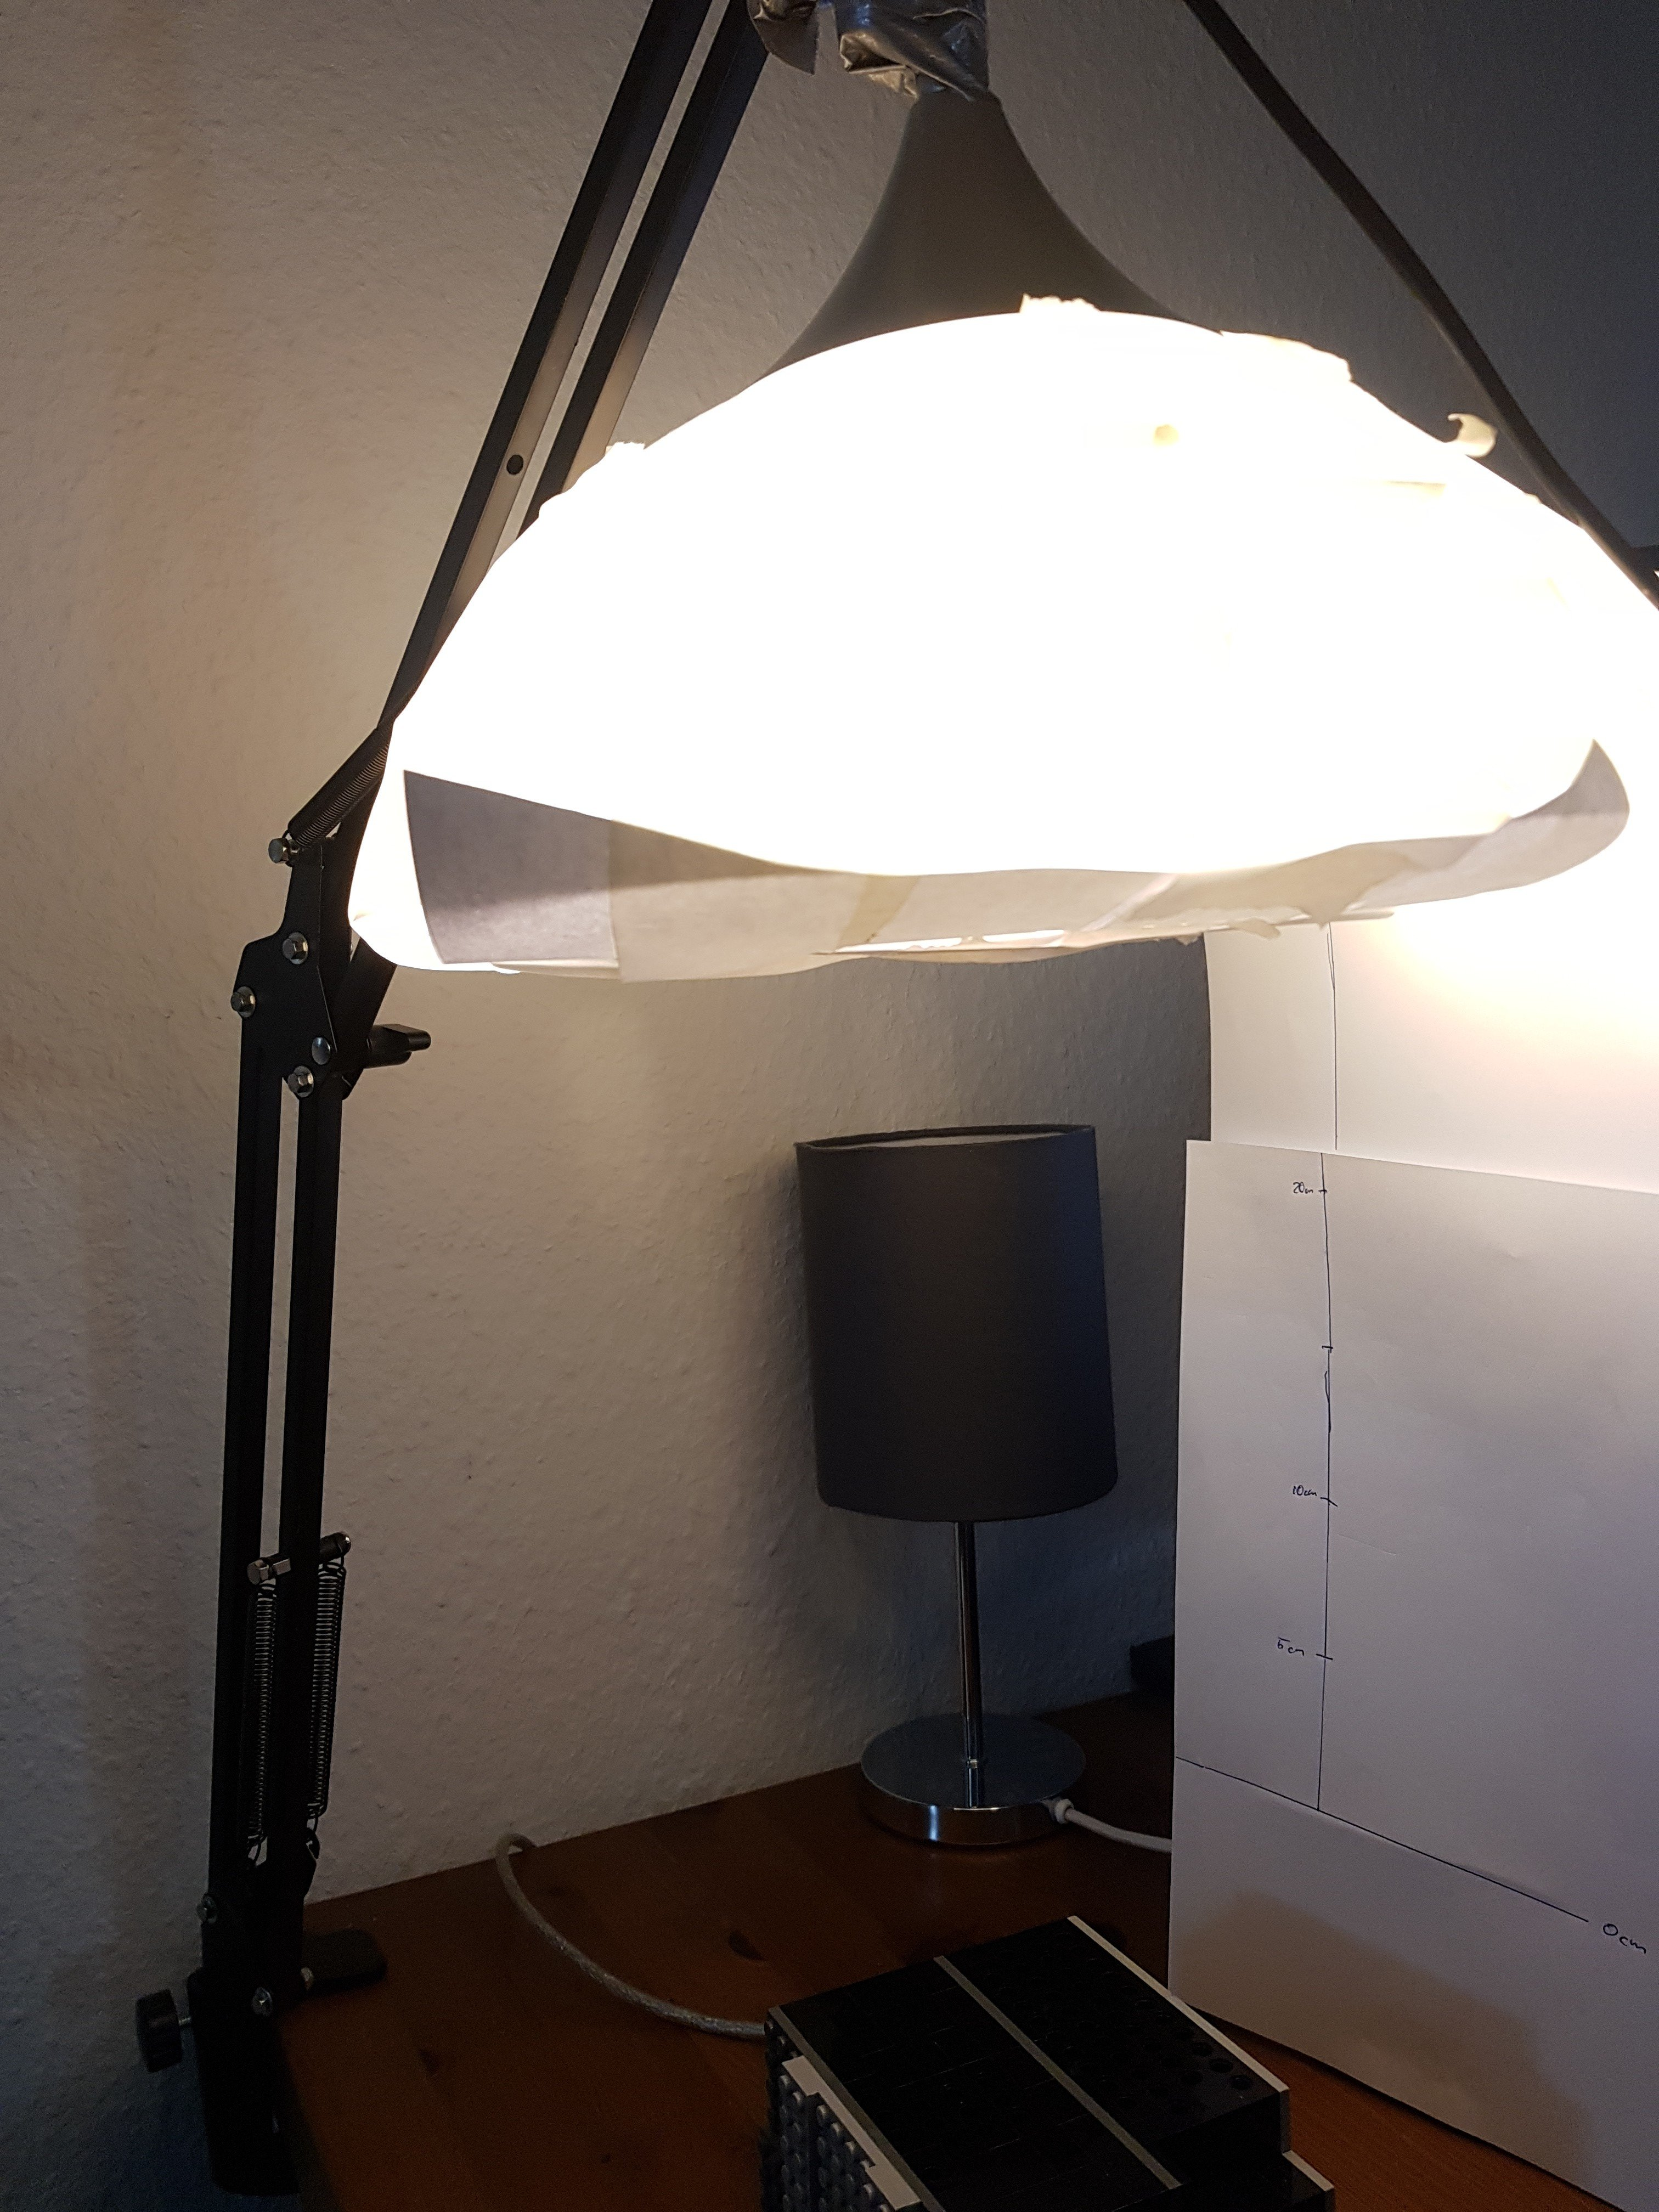
\includegraphics[width=0.33\linewidth]{images/light_low.jpeg}}\hfill%
\subfigure[Halbe Helligkeit]{\label{subfig:light_medium}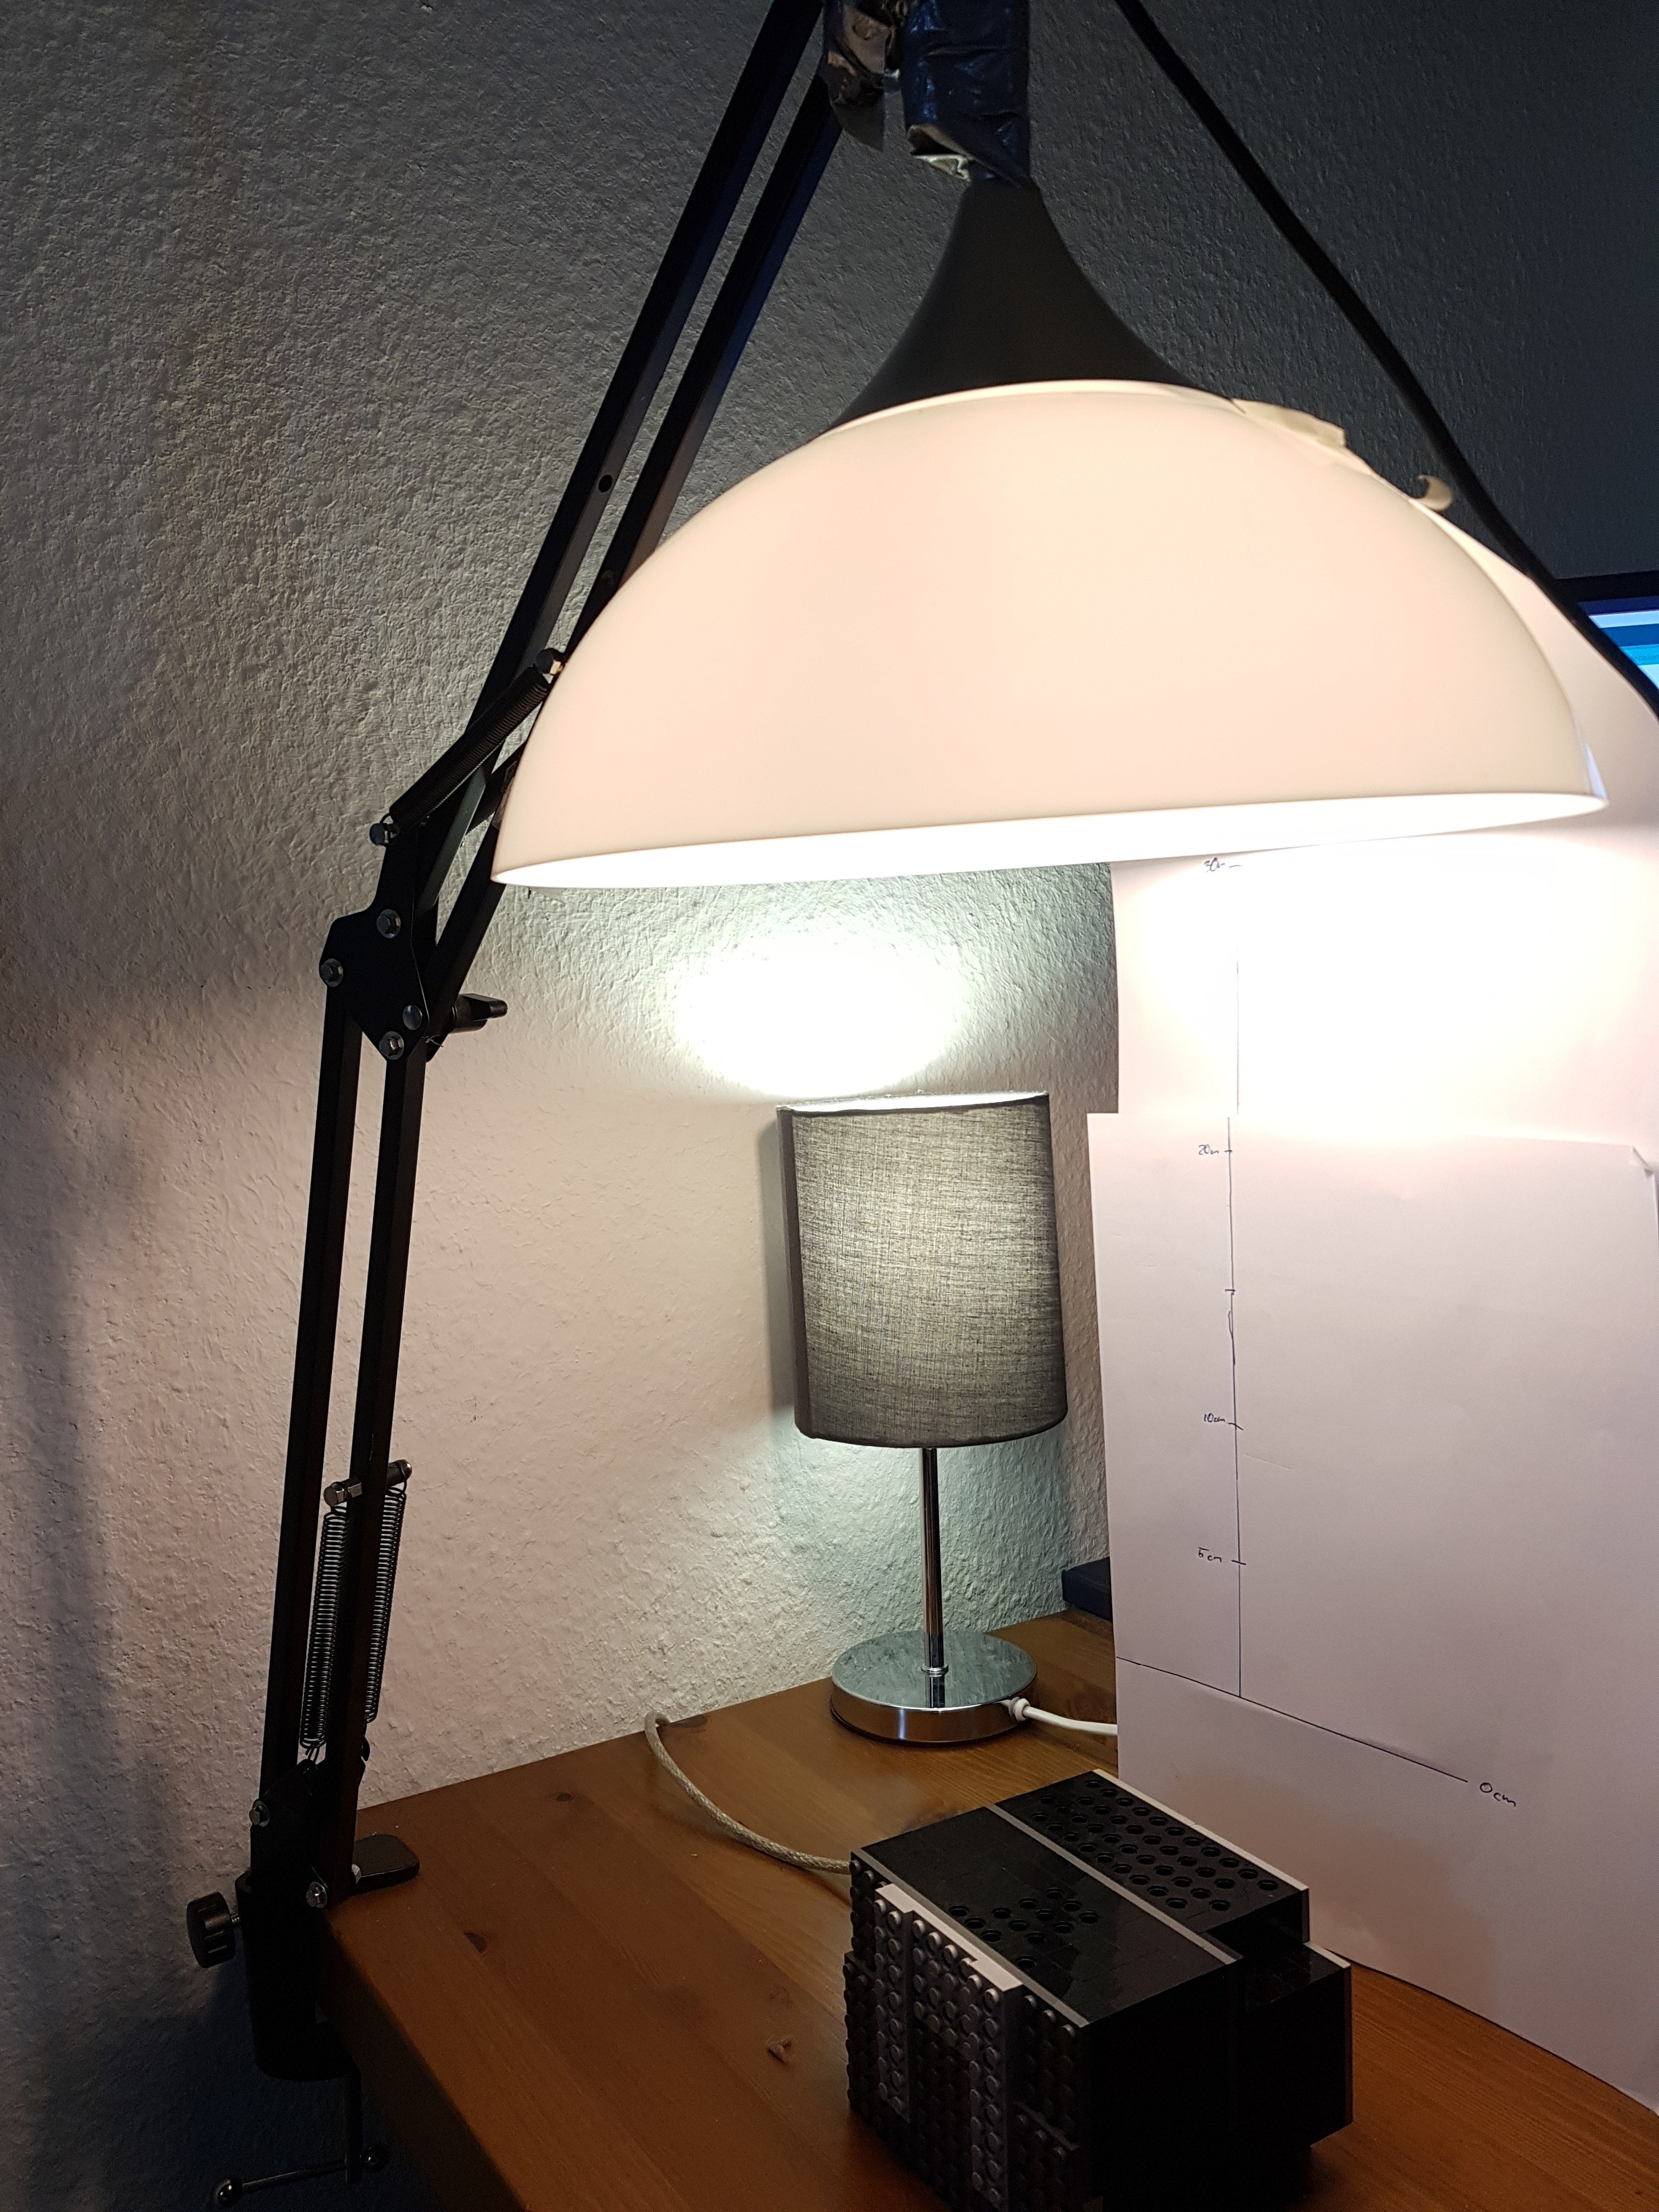
\includegraphics[width=0.33\linewidth]{images/light_medium.jpeg}}\hfill%
\subfigure[Hohe Helligkeit]{\label{subfig:light_high}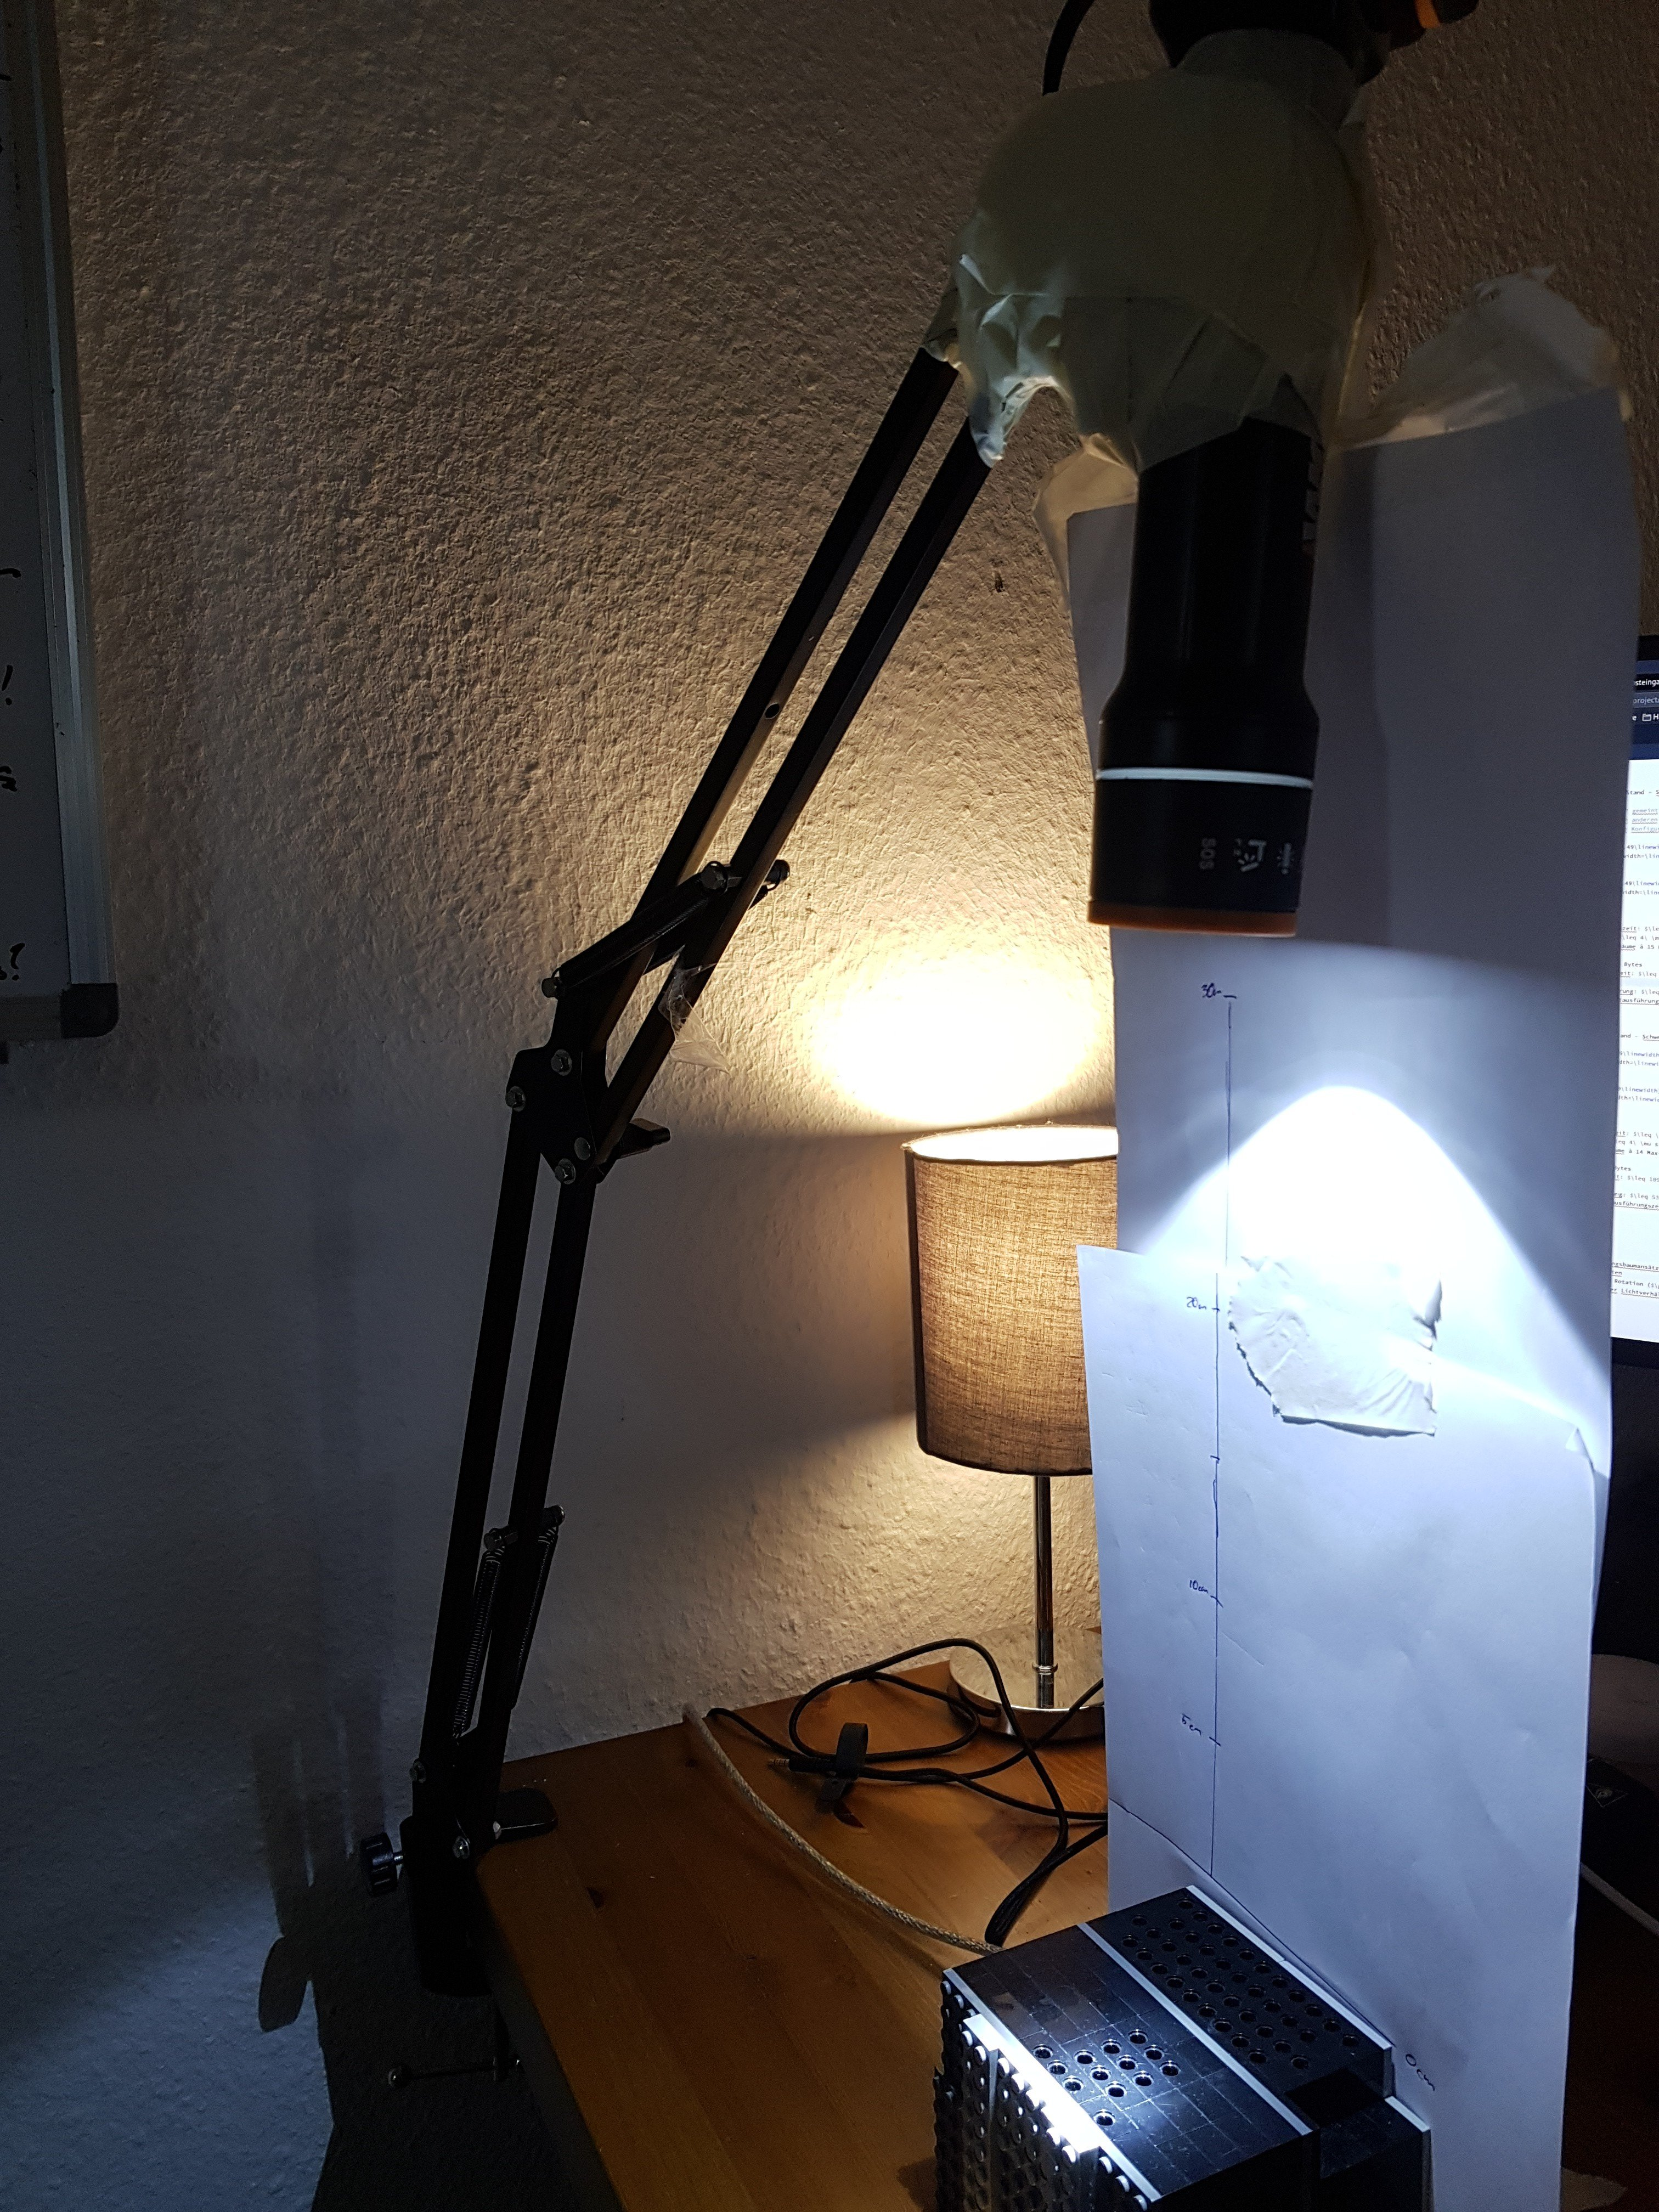
\includegraphics[width=0.33\linewidth]{images/light_high.jpeg}}%
}{Verschiedene Helligkeitsstufen unter denen die Gesten von \texttt{DymelData} aufgenommen wurden.}{fig:different_lights}
Jede Handgeste wurde unter jeder Konfiguration ca. 100 mal aufgenommen bei 90 Bildern pro Sekunde. Insgesamt wurden in 3 Lichtverhältnisse und 4 Distanzen, 6 verschiedene Gesten (Links nach Rechts,
Rechts nach Links, Oben nach Unten, Unten nach Oben und 2 Nullgesten) jeweils schnell und langsam aufgenommen. Die Gesten wurden in den Abständen 5 cm, 10 cm, 20 cm und 25 cm aufgenommen.
\newline
\newline
Die \glqq Geringe\grqq\ Helligkeit war im Durchschnitt bei ca. 140, \glqq Halbe\grqq\ Helligkeit bei ca. 659, \glqq Hohe\grqq\ Helligkeit bei ca. 908. Alle Helligkeiten haben das 3x3-Array
relativ gleichmäßig ausgeleuchtet. Bei den Lichtquellen \ref{subfig:light_low} und \ref{subfig:light_medium} wurde eine Schirmlampe verwendendet. Dadurch wurde das Licht relativ breit gestreut,
wodurch der Kontrast mit vergrößender Distanz abgenommen hat. Bei \ref{subfig:light_high} wurde eine Punktlichtquelle verwendet, wodurch der Kontrast über alle Distanzen sehr stark ist.
\newline
\newline
Insgesamt wurden 2 Typen von Nullgesten aufgenommen. Die erste Nullgeste geht \textit{Oben} rein, verschieden weit in Richtung \textit{Unten} und kehrt anschließend um, um bei \textit{Oben} wieder rauszukommen.
Die zweite Nullgeste geht \textit{Oben} rein, verschieden weit in Richtung \textit{Unten} und anschließend \textit{Rechts} wieder raus.
\newline
\newline
Die resultierenden Handgesten werden anschließend um 90°, 180° und 270° rotiert, um die equivalenten Nullgesten aus den anderen Richtungen zu inferieren. Insgesamt enstehen dadurch 19400 Nullgesten.
\newline
\newline
Um zu testen wie gut das Model sich gegenüber verschiedene Lichtverhältnisse generalisiert hat, ist es nötig mehr als nur 3 Helligkeitsstufen zu testen. Aus diesem Grund wurde aus der Gestenmenge mit
der Helligkeit \glqq Gering\grqq\ eine synthetische Testmenge generiert.
\newline
\newline
Dabei wurden jeweils 20 Duplikate der Datenmenge erstellt mit einem Helligkeitsoffset zwischen 50 und 1000 und einer Skalierung zwischen 0,5 und 10. Diese Datenmengen wurden zu einer Testmenge zusammengefügt.